\setcounter{section}{1}

\Needspace{5\baselineskip}
\hypertarget{umiux6570ux636e}{%
\section{UMI数据}\label{umiux6570ux636e}}

\Needspace{5\baselineskip}
\hypertarget{ux4e00umiux7684ux6838ux5fc3ux65b9ux6cd5}{%
\subsection{一、UMI的核心方法}\label{ux4e00umiux7684ux6838ux5fc3ux65b9ux6cd5}}

UMI用一个GoPro进行数据采集，包括一只手持夹爪及腕部视角相机，还通过两侧的镜子提供立体信息。UMI旨在用人类手持夹爪进行操作的方式采集数据，从而既具备人类操作的灵活性，又与机器人操作同构且本体无关，还可以让数据采集不再局限在封闭的数采厂，使得数据多样化程度更高、获取成本更低。

\begin{figure}[htbp]
\centering
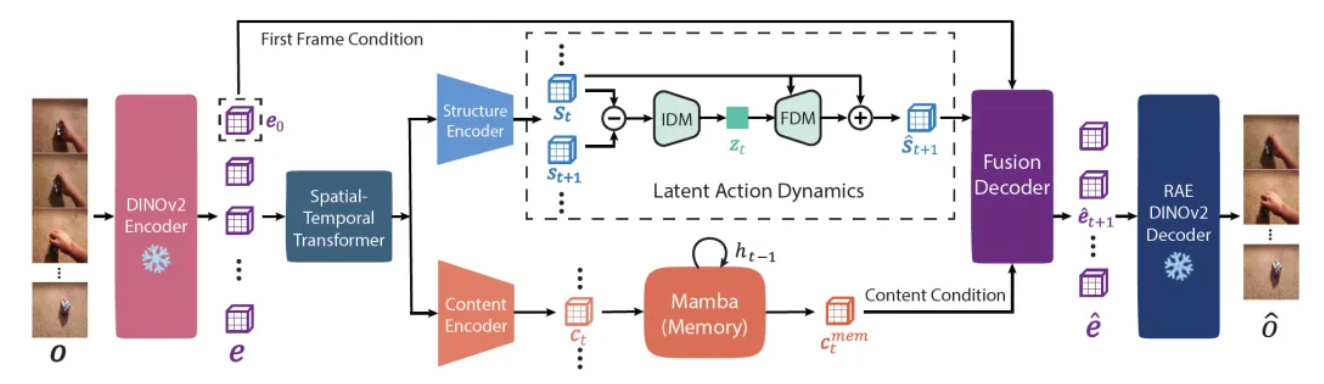
\includegraphics{images/image-0053.png}
\caption{UMI 手持数据采集设备}
\end{figure}

UMI采集的数据包括相机拍摄的图像、夹爪开合度（连续而非离散）以及相对末端执行器的位姿轨迹的数据。其中，图像采用腕部第一视角相机作为唯一的观测点；相对位姿表示解除了对特定机器人基坐标系的依赖，实现了本体无关性，用于机器人时只需将相对轨迹转化为关节指令即可。

\Needspace{5\baselineskip}
\hypertarget{ux4e8cumiux6570ux636eux91c7ux96c6ux7684ux6539ux8fdbux4e0eux8d28ux91cfux63a7ux5236}{%
\subsection{二、UMI数据采集的改进与质量控制}\label{ux4e8cumiux6570ux636eux91c7ux96c6ux7684ux6539ux8fdbux4e0eux8d28ux91cfux63a7ux5236}}

\Needspace{5\baselineskip}
\hypertarget{ux4e00umiux8bbeux5907ux7684ux6539ux8fdbux65b9ux5411}{%
\subsubsection{（一）UMI设备的改进方向}\label{ux4e00umiux8bbeux5907ux7684ux6539ux8fdbux65b9ux5411}}

\begin{enumerate}
\def\labelenumi{\arabic{enumi}.}
\item
  制造工艺调整、轻量化、易用性提升和鲁棒性提升。
\item
  针对部分操作中相机视野被遮挡，导致部分精细操作数据不可用的问题，可增加更多视角，但需要注意处理好具身差异。
\item
  针对触觉和力的数据缺失的问题，可增加相应传感器。
\item
  末端从简单的平行夹爪演进到更通用、更灵巧的末端形态。
\end{enumerate}

\Needspace{5\baselineskip}
\hypertarget{ux4e8cumiux6570ux636eux91c7ux96c6ux7684ux8d28ux91cfux63a7ux5236}{%
\subsubsection{（二）UMI数据采集的质量控制}\label{ux4e8cumiux6570ux636eux91c7ux96c6ux7684ux8d28ux91cfux63a7ux5236}}

大规模数据采集中，常出现无效数据，如操作速度过快，超出了机器臂的物理极限；或者将手伸到机械臂无法复现的位置，导致运动学逆解失败。有时数据中还有大量无意义的片段，如反复拿起又放下同一个物体、打开开关后却没有进行下一步操作等。数据质量控制非常重要。如能实现实时质量控制，则相较于采集完毕后统一进行质量检查将能减少许多浪费。

另外，数据的难点不在于单纯的获取，而在于让获取的数据能用于模型训练。这需要数据和模型协同进化，将采集的数据用于模型迭代，发现问题后及时调整优化数据采集策略。

\Needspace{5\baselineskip}
\hypertarget{ux4e09genux7cfbux5217ux57faux4e8eumiux6570ux636eux9884ux8badux7ec3ux7684scaling-law}{%
\subsection{三、GEN系列：基于UMI数据预训练的Scaling Law}\label{ux4e09genux7cfbux5217ux57faux4e8eumiux6570ux636eux9884ux8badux7ec3ux7684scaling-law}}

Generalist的GEN系列模型利用大规模UMI数据进行具身原生预训练。从GEN-0的27万小时，到GEN-1的50万小时，再到GEN-1.5更大规模的数据，模型能力不断提升。

\Needspace{5\baselineskip}
在GEN-0的预训练中，Generalist发现模型的表现与计算、数据和参数的关系可以体现Scaling Law：

\begin{figure}[htbp]
\centering
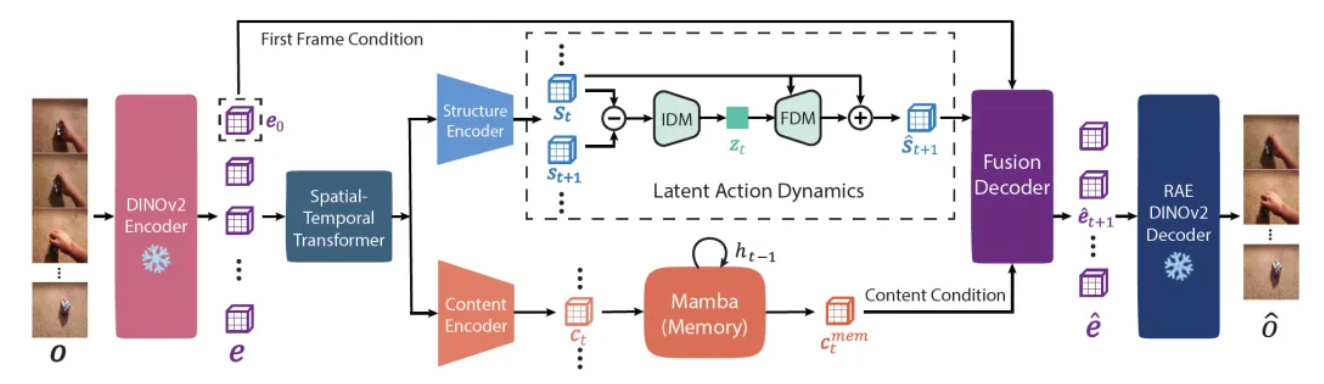
\includegraphics{images/image-0054.png}
\caption{GEN-0 随数据量和计算量扩展的性能曲线}
\end{figure}

\begin{figure}[htbp]
\centering
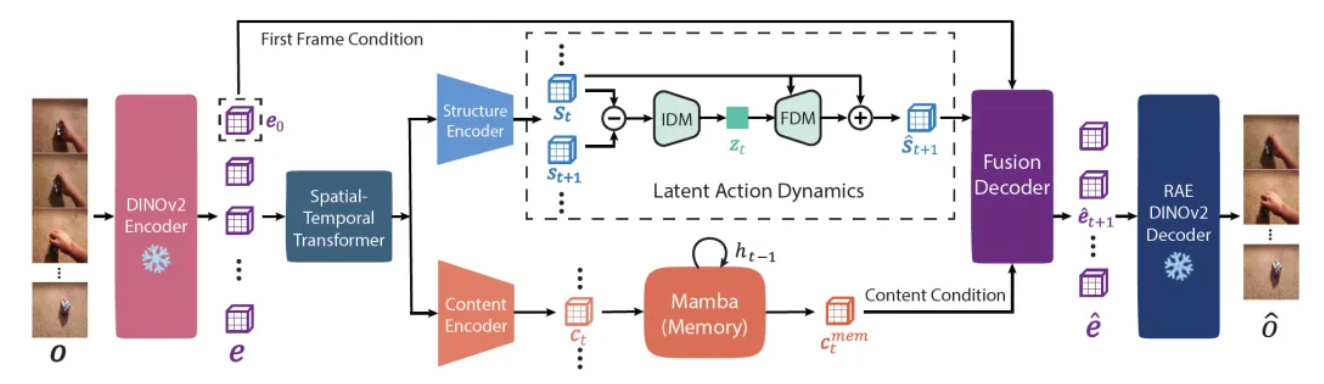
\includegraphics{images/image-0055.png}
\caption{GEN-0 随任务集合扩展的性能曲线}
\end{figure}

而到GEN-1.5，模型开始呈现出上下文学习能力。给模型看单次较短的示范，把它放进上下文窗口，机器人就能立刻做这件事，全程不需要更新梯度。仿真里录制的示范也可以（而GEN-1.5没有用仿真数据训练过）。物理提示可以像文本提示一样拼接，且模型可以通过类比的方式用示范里没有直接出现过的工具和策略进行操作。

如图是GEN-1.5预训练中损失持续呈下降趋势的曲线。

\begin{figure}[htbp]
\centering
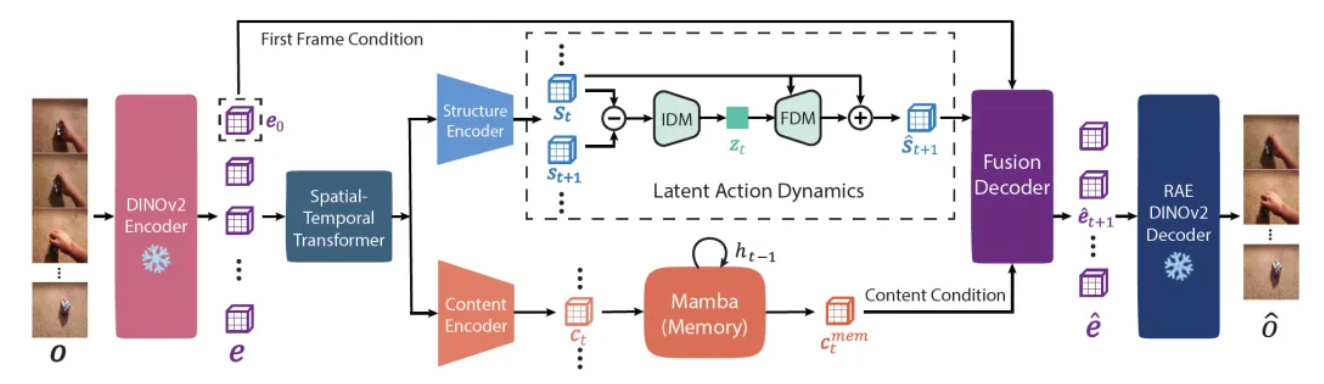
\includegraphics{images/image-0056.png}
\caption{GEN-1.5 的训练损失曲线}
\end{figure}

\Needspace{5\baselineskip}
\hypertarget{ux56dbumiux7684ux884dux751fux4f53ux901aux8fc7ux53efux7a7fux6234ux5916ux9aa8ux9abcux91c7ux96c6ux6570ux636e}{%
\subsection{四、UMI的衍生体：通过可穿戴外骨骼采集数据}\label{ux56dbumiux7684ux884dux751fux4f53ux901aux8fc7ux53efux7a7fux6234ux5916ux9aa8ux9abcux91c7ux96c6ux6570ux636e}}

随着机器人末端从平行夹爪向多指灵巧手发展，UMI的思路也开始从手持夹爪进一步延伸到可穿戴外骨骼等。其核心仍然是利用人类直接操作真实物体来采集数据，但通过外骨骼将人的手部动作约束和映射到机器人灵巧手的可执行空间，从而减少人手与机器人手之间的具身差异。

以DexUMI为例，它为不同机器人灵巧手设计对应的手部外骨骼，使人可以直接完成抓取、旋拧、工具使用等复杂操作，同时记录多指动作和触觉信息。相比于先采集裸手动作再进行retargeting，外骨骼能够在数据采集阶段就缩小运动学差异。针对采集时看到``人手+外骨骼''、部署时看到机器人手所带来的视觉差异，DexUMI还通过视觉处理将采集画面转换得更接近机器人部署时的观测。

后续的一些工作也采用了类似思路，但进一步强调采集端与机器人端的协同设计。如TwinDEX的三指外骨骼与机器人三指手在运动学结构上尽可能保持一致，从硬件层面减少动作映射和retargeting的复杂度。数据采集设备正从简单夹爪向多指灵巧手发展，并越来越多地通过软硬件协同设计，在数据采集阶段就主动缩小Embodiment Gap。

\FloatBarrier
\Needspace{5\baselineskip}
\hypertarget{ux53c2ux8003ux6587ux732e-163}{%
\subsection{参考文献}\label{ux53c2ux8003ux6587ux732e-163}}

\vspace{0.25em}
\begin{itemize}
\tightlist
\item
  Chi, C., Xu, Z., Pan, C., et al.~(2024). \href{https://arxiv.org/abs/2402.10329}{Universal Manipulation Interface: In-The-Wild Robot Teaching Without In-The-Wild Robots}. arXiv:2402.10329.
\item
  Rayyan, O., Abanes, J., Hafez, M., Tzes, A., \& Abu-Dakka, F. (2025). \href{https://arxiv.org/abs/2509.18757}{MV-UMI: A Scalable Multi-View Interface for Cross-Embodiment Learning}. arXiv:2509.18757.
\item
  Liu, F., Li, C., Qin, Y., Xu, J., Abbeel, P., \& Chen, R. (2025). \href{https://arxiv.org/abs/2504.06156}{ViTaMIn: Learning Contact-Rich Tasks Through Robot-Free Visuo-Tactile Manipulation Interface}. arXiv:2504.06156.
\item
  Xu, M., Zhang, H., Hou, Y., et al.~(2025). \href{https://arxiv.org/abs/2505.21864}{DexUMI: Using Human Hand as the Universal Manipulation Interface for Dexterous Manipulation}. arXiv:2505.21864.
\item
  X Square Robot. (2026). \href{https://x2robot.com/en/pages/twindex}{TwinDEX --- Dexterous. Consistent. Scalable}. Project page.
\item
  Lin, F., Hu, Y., Sheng, P., Wen, C., You, J., \& Gao, Y. (2025). \href{https://proceedings.iclr.cc/paper_files/paper/2025/hash/88b7b2c896506daabc8d3fd587055167-Abstract-Conference.html}{Data Scaling Laws in Imitation Learning for Robotic Manipulation}. ICLR.
\item
  Generalist Team. (2025). \href{https://generalistai.com/blog/gen-0}{GEN-0: Embodied Foundation Models That Scale with Physical Interaction}. Generalist.
\item
  Generalist Team. (2026). \href{https://generalistai.com/blog/gen-1}{GEN-1: Scaling Embodied Foundation Models to Mastery}. Generalist.
\item
  Generalist Team. (2026). \href{https://generalistai.com/blog/gen-1.5}{GEN-1.5: Embodied Foundation Models are One-Shot Learners}. Generalist.
\end{itemize}

\clearpage
